\documentclass[UTF8,a4paper,11pt,fontset=windows]{ctexart}
\usepackage[margin=2.1cm]{geometry}
\usepackage{graphicx,float,booktabs,tabularx,fancyhdr,xurl,fvextra}
\usepackage[hidelinks]{hyperref}
\setlength{\parskip}{.25em}\setlength{\emergencystretch}{2em}
\renewcommand{\arraystretch}{1.2}\raggedbottom
\ctexset{section={format={\large\bfseries\raggedright},beforeskip=1.2ex,afterskip=.6ex}}
\linespread{1.12}
\pagestyle{fancy}\fancyhf{}\fancyhead[L]{互联网数据库开发 · 绿茵数据团队}
\fancyhead[R]{绿茵视界}\fancyfoot[C]{\thepage}\setlength{\headheight}{14pt}
\begin{document}
\begin{titlepage}\thispagestyle{empty}\centering
\vspace*{.6cm}
\includegraphics[width=.43\textwidth]{../../figures/nankai_logo_color.png}
\vspace{.9cm}\rule{.88\textwidth}{.8pt}\par\vspace{.55cm}
{\fontsize{27pt}{35pt}\selectfont\bfseries 互联网数据库开发课程设计\par}
\vspace{.65cm}{\fontsize{21pt}{29pt}\selectfont\bfseries 实现文档\par}
\vspace{.55cm}\rule{.88\textwidth}{.8pt}\par\vspace{1.1cm}
{\Large 绿茵视界\par 世界杯赛事数据与球迷互动平台\par}
\vspace{.65cm}{\large 绿茵数据团队\par 黄奕浩\quad 2413581\quad 组长\par 王乐之\quad 2411302\par}
\end{titlepage}
\section{公共模块结构}
本人负责公共及社区9张表：用户、开发团队、成员、公告、作业文件、审计、通知、话题和评论。Model维护约束及关系，Controller检查身份和处理请求，View负责表单与转义后的内容。页面使用海军蓝、球场绿与浅色内容区，统一文字层级、表格垂直对齐和手机布局。

\begin{figure}[H]\centering
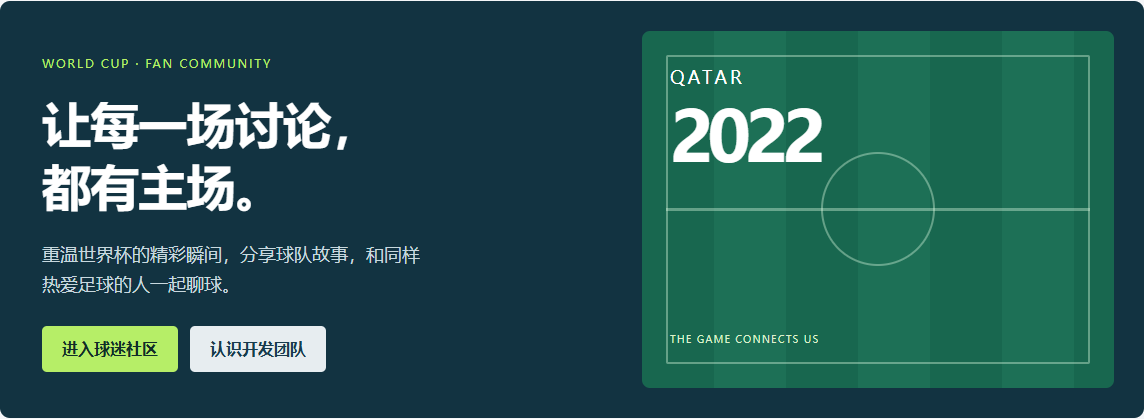
\includegraphics[width=\linewidth,height=.33\textheight,keepaspectratio]{../../figures/01_home.png}
\caption{世界杯主题首页}
\end{figure}

\section{账户与开发团队}
注册校验用户名、邮箱、密码及图形验证码，账户角色由服务器设为member。登录验证密码哈希，后台在应用和管理员基类检查admin角色。site/me返回登录状态、用户编号、用户名和角色，供赛事模块复用。个人编辑从会话确定资料，不使用请求中的用户编号定位编辑对象。

开发团队与国家队分别存储，团队页仅展示两名开发者。管理员可以编辑团队及成员介绍，保存后前台读取更新内容。普通注册用户可维护个人资料，其身份不加入开发团队展示。

\begin{figure}[H]\centering

\includegraphics[width=\linewidth,height=.27\textheight,keepaspectratio]{../../figures/02_developers.png}
\caption{开发团队展示}
\end{figure}

\begin{figure}[H]\centering
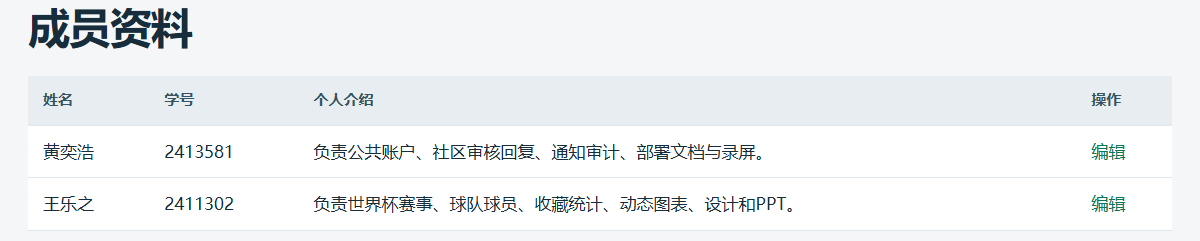
\includegraphics[width=\linewidth,height=.24\textheight,keepaspectratio]{../../figures/04_member_admin.png}
\caption{后台成员维护}
\end{figure}

\section{话题、评论与回复}
球迷社区支持关键词搜索、分页、发布和编辑话题。话题可选关联比赛，MatchReference提供比赛选择项。作者编辑后状态重新变为pending；撤下使用POST并校验所有权。公开页只查询published状态，未审内容返回404。

评论从当前登录会话确定作者，回复对象必须属于同一话题且已公开。表单验证通过后保存，管理员审核后显示。正文和回复使用Html转义；父评论撤下后，其回复从公开列表中隐藏。

\begin{figure}[H]\centering
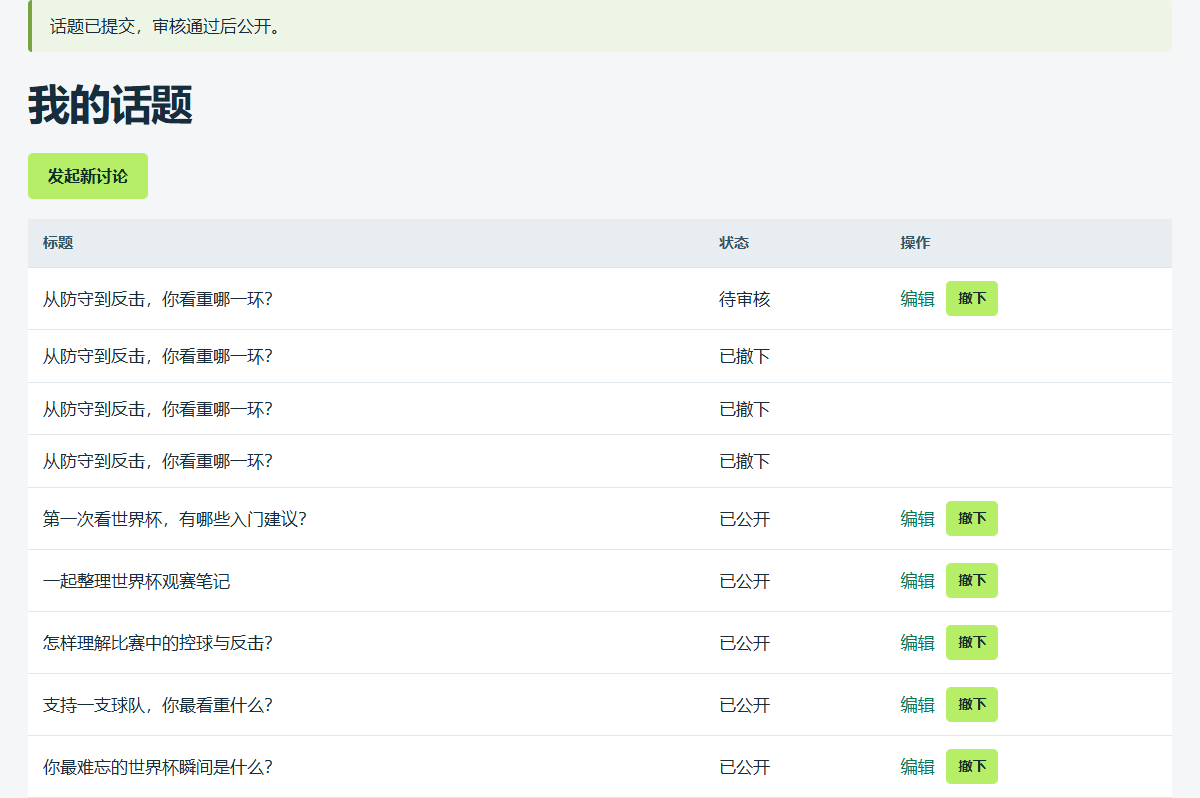
\includegraphics[width=\linewidth,height=.25\textheight,keepaspectratio]{../../figures/05_post_pending.png}
\caption{话题提交后的待审核状态}
\end{figure}

\begin{figure}[H]\centering
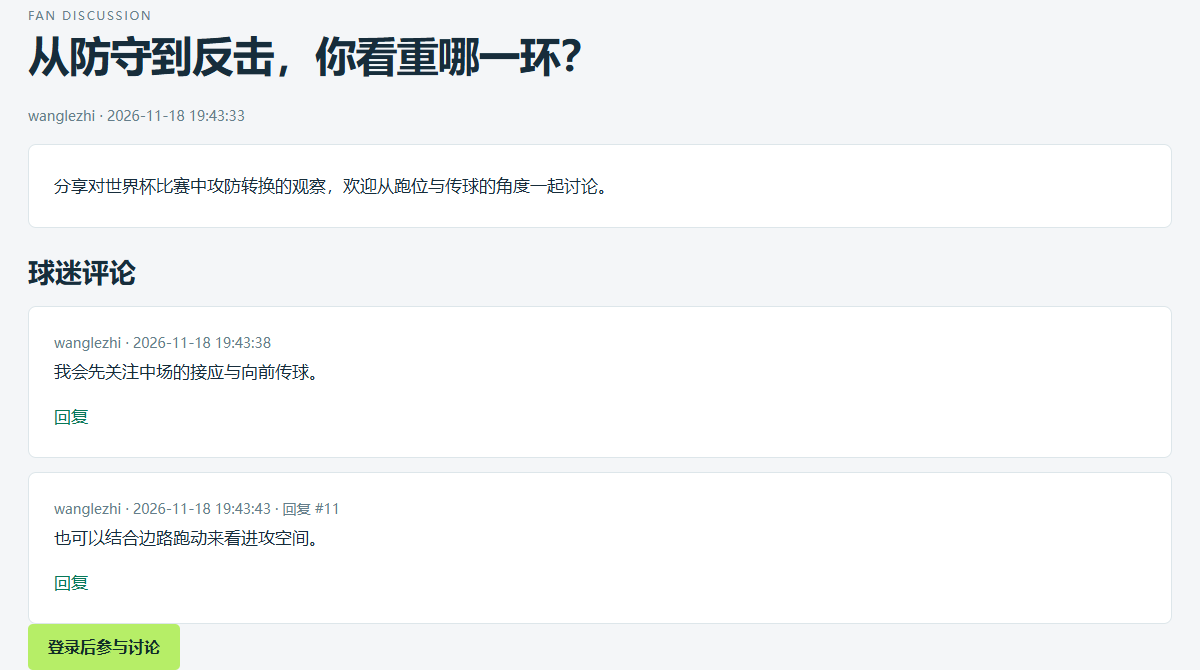
\includegraphics[width=\linewidth,height=.30\textheight,keepaspectratio]{../../figures/07_comments_reply.png}
\caption{话题评论与回复}
\end{figure}

\section{审核、邮件与操作日志}
后台按话题和评论分开管理，支持待审、通过、驳回和撤下。审核保存后通过NotificationService生成数据库通知和本机EML，投递失败保留failed状态。通知预览按记录编号读取，页面只对管理员开放。SMTP参数在本机配置，默认文件投递。

AdminController在后台写操作结束后调用AuditLog，社区提交与撤下也记录对象。日志包含操作者、动作、对象编号和时间，文件日志记录登录事件及首页性能标记。

\begin{figure}[H]\centering
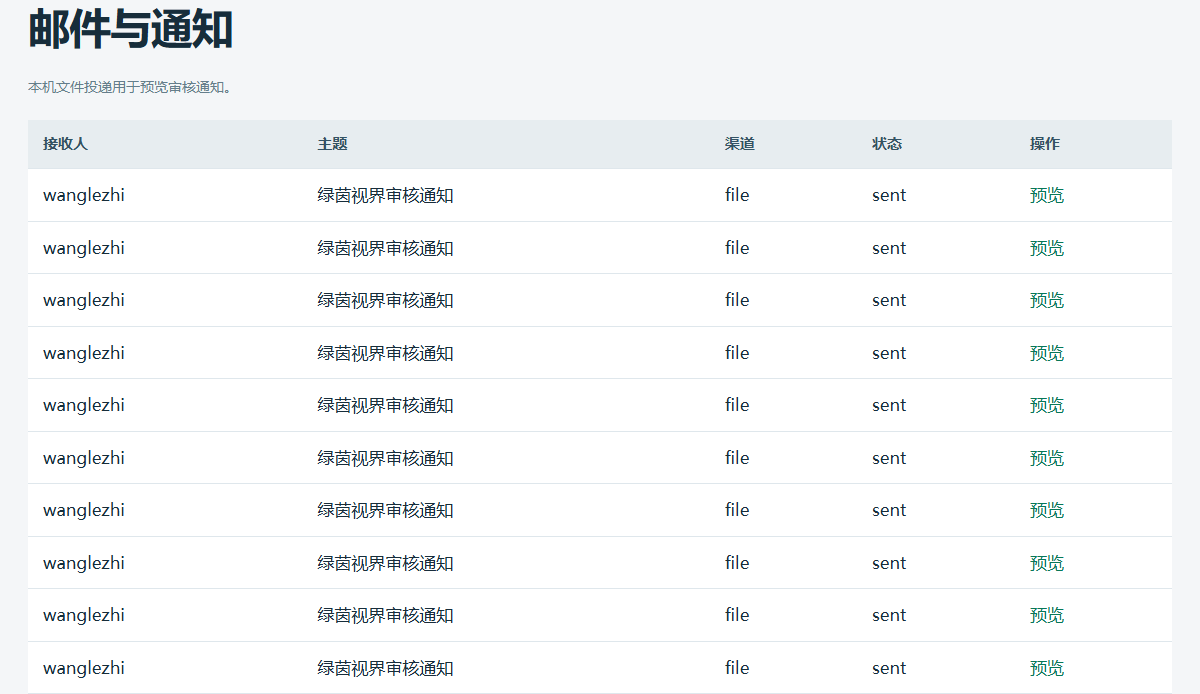
\includegraphics[width=\linewidth,height=.25\textheight,keepaspectratio]{../../figures/08_notifications.png}
\caption{通知投递记录}
\end{figure}

\begin{figure}[H]\centering

\includegraphics[width=\linewidth,height=.24\textheight,keepaspectratio]{../../figures/09_mail_preview.png}
\caption{通知预览}
\end{figure}

\begin{figure}[H]\centering
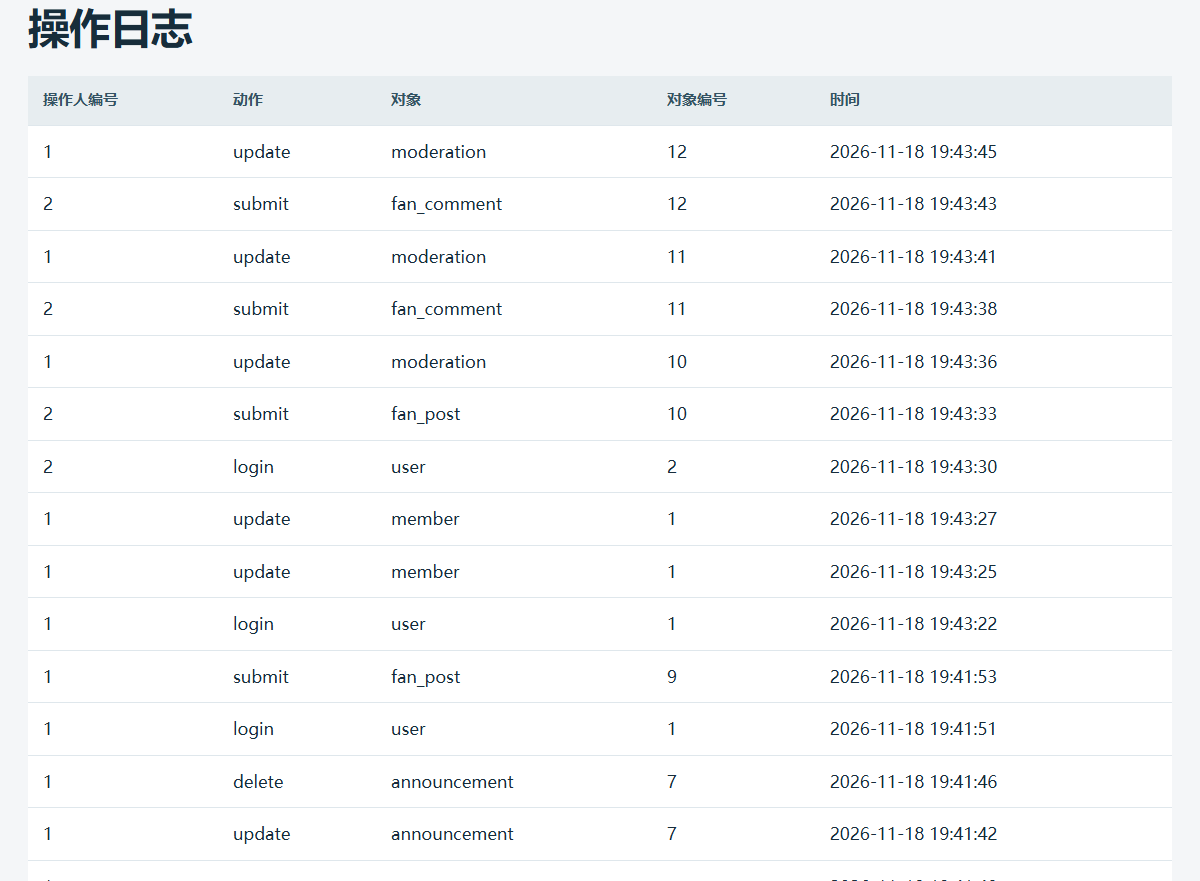
\includegraphics[width=\linewidth,height=.28\textheight,keepaspectratio]{../../figures/10_audit.png}
\caption{公共操作日志}
\end{figure}

请求调试记录请求方法、异步标志和登录状态，首页使用beginProfile与endProfile记录执行区间。文件日志按业务分类输出，关闭请求变量附带记录。

\begin{figure}[H]\centering
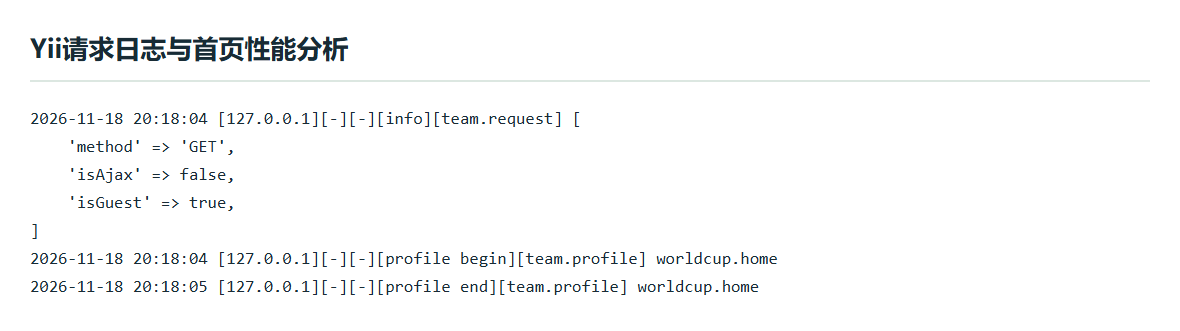
\includegraphics[width=\linewidth,height=.26\textheight,keepaspectratio]{../../figures/18_request_profile.png}
\caption{请求调试与性能日志}
\end{figure}

\section{公告与作业下载}
公告采用草稿、发布、撤下状态，前台查询同时检查发布时间。删除限定POST，表单保留CSRF。文件登记保存范围、相对路径与SHA256；下载只接收记录编号，先解析路径边界，再检查文件存在和摘要，最后返回附件。下载目录分别为data/team和data/personal。

\begin{figure}[H]\centering
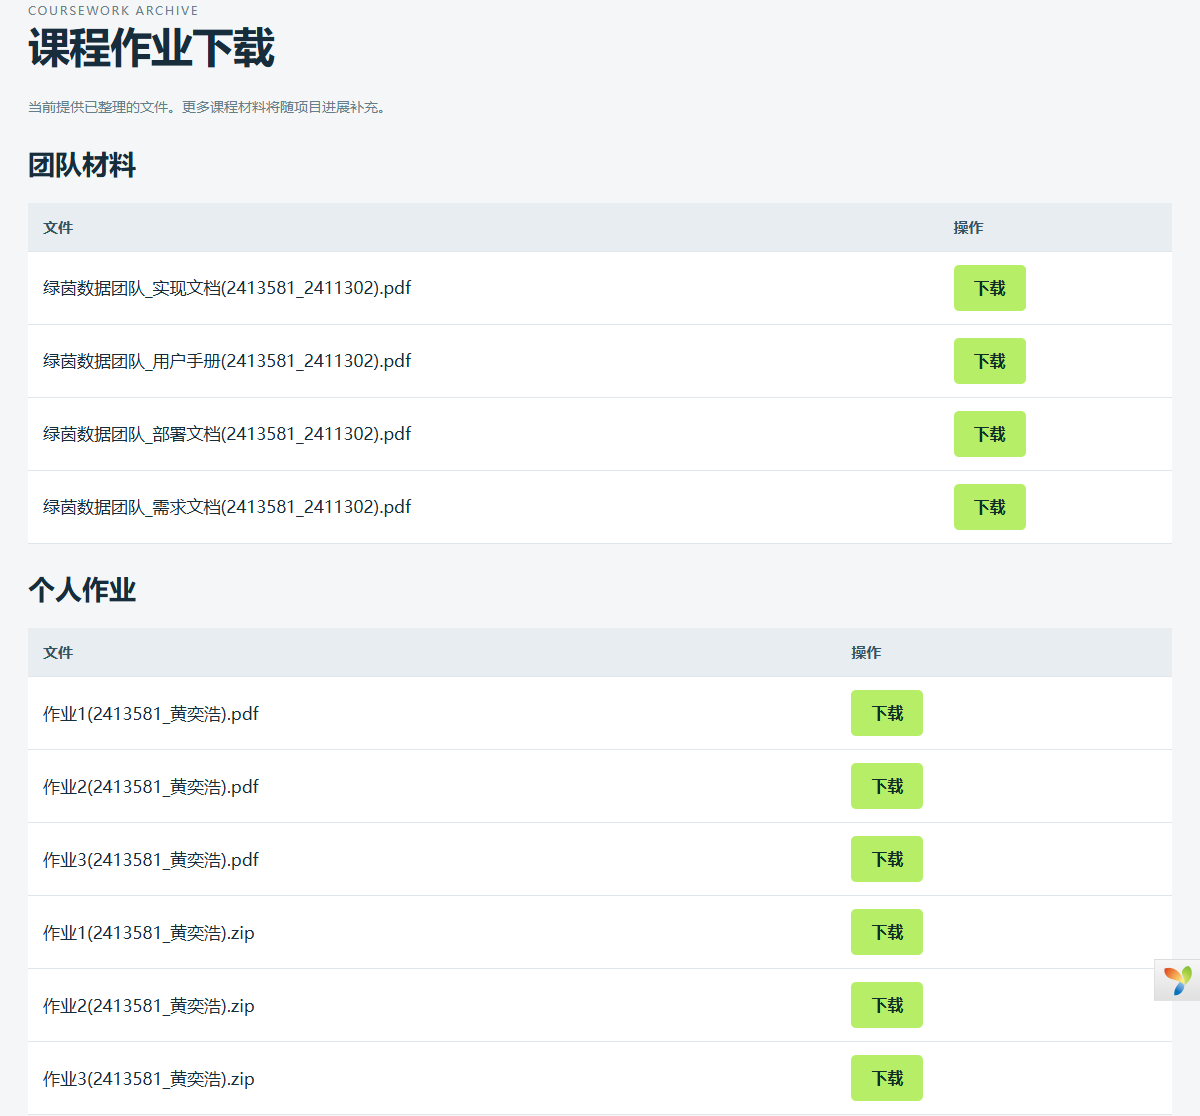
\includegraphics[width=\linewidth,height=.31\textheight,keepaspectratio]{../../figures/11_downloads.png}
\caption{作业下载中心}
\end{figure}

\section{代码、目录与提交}
项目按MVC组织，公共接口、业务文件和提交记录如下。Tower任务总览及详情截图在项目建立并分配任务后汇入本节。

\begin{figure}[H]\centering
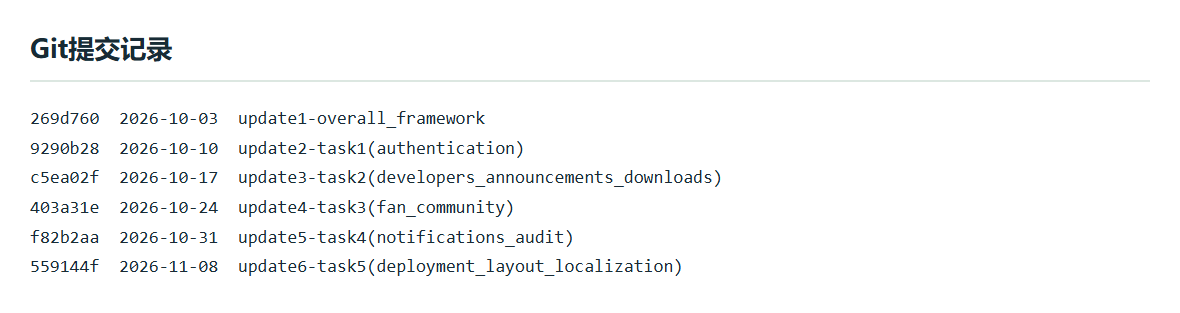
\includegraphics[width=\linewidth,height=.24\textheight,keepaspectratio]{../../figures/15_git.png}
\caption{Git提交记录}
\end{figure}

\begin{figure}[H]\centering
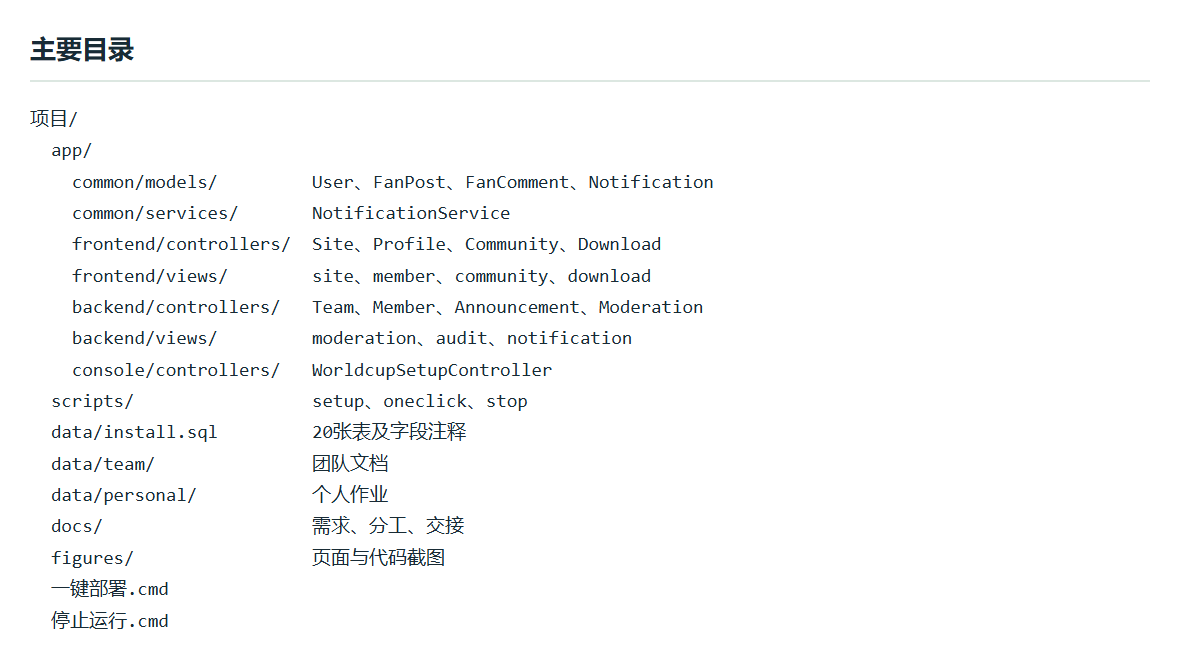
\includegraphics[width=\linewidth,height=.25\textheight,keepaspectratio]{../../figures/16_tree.png}
\caption{主要目录}
\end{figure}

\begin{figure}[H]\centering
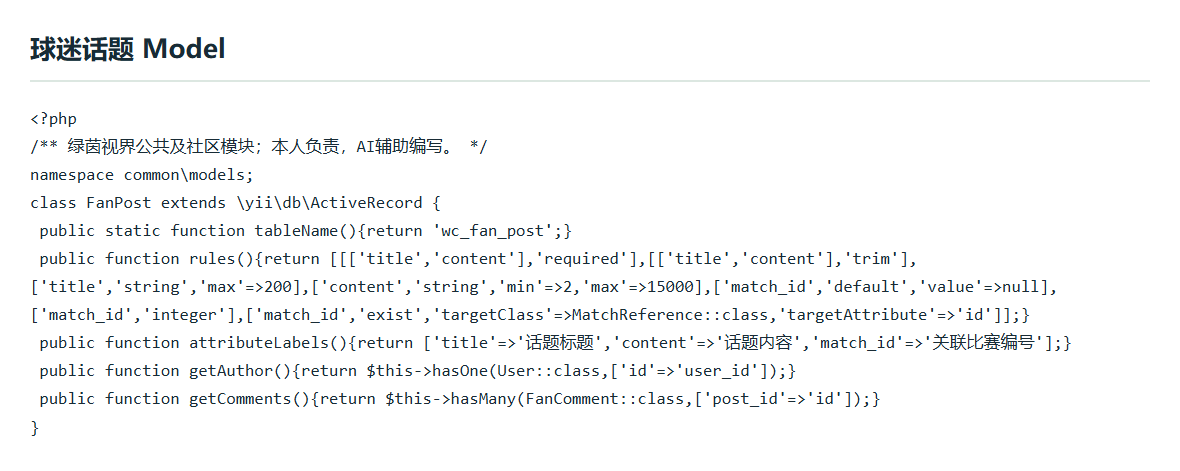
\includegraphics[width=\linewidth,height=.28\textheight,keepaspectratio]{../../figures/17_code.png}
\caption{社区Model代码}
\end{figure}

\section{部署与接口交接}
一键部署完成独立建库、随机口令、配置、结构导入、公共样例与服务启动，停止脚本保留数据。赛事模块可使用公共用户、管理员基类、日志和通知服务。比赛表录入后，社区发帖界面自动提供关联选项。赛事查询、收藏、积分射手榜和图表待王乐之接入；完整PPT和录屏在全组页面齐备后整合。

\end{document}
